%\documentclass[10pt,handout]{beamer}
\documentclass[11pt]{beamer}\usepackage[]{graphicx}\usepackage[]{color}
%% maxwidth is the original width if it is less than linewidth
%% otherwise use linewidth (to make sure the graphics do not exceed the margin)
\makeatletter
\def\maxwidth{ %
  \ifdim\Gin@nat@width>\linewidth
    \linewidth
  \else
    \Gin@nat@width
  \fi
}
\makeatother

\definecolor{fgcolor}{rgb}{0.196, 0.196, 0.196}
\newcommand{\hlnum}[1]{\textcolor[rgb]{0.063,0.58,0.627}{#1}}%
\newcommand{\hlstr}[1]{\textcolor[rgb]{0.063,0.58,0.627}{#1}}%
\newcommand{\hlcom}[1]{\textcolor[rgb]{0.588,0.588,0.588}{#1}}%
\newcommand{\hlopt}[1]{\textcolor[rgb]{0.196,0.196,0.196}{#1}}%
\newcommand{\hlstd}[1]{\textcolor[rgb]{0.196,0.196,0.196}{#1}}%
\newcommand{\hlkwa}[1]{\textcolor[rgb]{0.231,0.416,0.784}{#1}}%
\newcommand{\hlkwb}[1]{\textcolor[rgb]{0.627,0,0.314}{#1}}%
\newcommand{\hlkwc}[1]{\textcolor[rgb]{0,0.631,0.314}{#1}}%
\newcommand{\hlkwd}[1]{\textcolor[rgb]{0.78,0.227,0.412}{#1}}%
\let\hlipl\hlkwb

\usepackage{framed}
\makeatletter
\newenvironment{kframe}{%
 \def\at@end@of@kframe{}%
 \ifinner\ifhmode%
  \def\at@end@of@kframe{\end{minipage}}%
  \begin{minipage}{\columnwidth}%
 \fi\fi%
 \def\FrameCommand##1{\hskip\@totalleftmargin \hskip-\fboxsep
 \colorbox{shadecolor}{##1}\hskip-\fboxsep
     % There is no \\@totalrightmargin, so:
     \hskip-\linewidth \hskip-\@totalleftmargin \hskip\columnwidth}%
 \MakeFramed {\advance\hsize-\width
   \@totalleftmargin\z@ \linewidth\hsize
   \@setminipage}}%
 {\par\unskip\endMakeFramed%
 \at@end@of@kframe}
\makeatother

\definecolor{shadecolor}{rgb}{.97, .97, .97}
\definecolor{messagecolor}{rgb}{0, 0, 0}
\definecolor{warningcolor}{rgb}{1, 0, 1}
\definecolor{errorcolor}{rgb}{1, 0, 0}
\newenvironment{knitrout}{}{} % an empty environment to be redefined in TeX

\usepackage{alltt}
%\documentclass[11pt, handout]{beamer}
%\usepackage{handoutWithNotes}
%\usepackage{pgfpages}
\usepackage{etex} % helps fix \newdimen error which is cause when ctable is loaded with other packages
\usepackage{comment}
\usepackage{amsmath,amsthm,amssymb}
\newtheorem{rcode}{R code}[section]
\usepackage{url}

%\usepackage[usenames]{xcolor}
\usepackage{color, colortbl}
\usepackage{tikz}
\usepackage[utf8]{inputenc}
\usepackage[T1]{fontenc}
\usepackage{ae}
%\usepackage{aeguill}
\usepackage{ctable}


\usetikzlibrary{shapes.geometric, arrows,shapes.symbols,decorations.pathreplacing}
\tikzstyle{startstop} = [rectangle, rounded corners, minimum width=3cm, minimum height=1cm, draw=black, fill=pinkish,text width=3.5cm]
\tikzstyle{startstop2} = [rectangle, rounded corners, minimum width=3cm, minimum height=1cm, draw=black, fill=background,text width=2.5cm]
\tikzstyle{startstop3} = [rectangle, rounded corners, minimum width=3cm, minimum height=1cm, draw=black, fill=beige,text width=3.0cm]
\tikzstyle{io} = [trapezium, trapezium left angle=70, trapezium right angle=110, minimum width=2cm, minimum height=1cm, text centered, draw=black, fill=blue!30,text width=1.5cm]
\tikzstyle{process} = [rectangle, minimum width=1cm, minimum height=1cm, text centered, draw=black, fill=orange!30,text width=2cm]
\tikzstyle{decision} = [diamond, minimum width=2cm, minimum height=1cm, text centered, draw=black, fill=green!30]
\tikzstyle{arrow} = [thick,->,>=stealth]
\tikzstyle{both} = [thick,<->,>=stealth, red]

\tikzset{myshade/.style={minimum size=.4cm,shading=radial,inner color=white,outer color={#1!90!gray}}}
\newcommand\mycirc[1][]{\tikz\node[circle,myshade=#1]{};}
\newcommand\myrect[1][]{\tikz\node[rectangle,myshade=#1]{};}
\newcommand\mystar[1][]{\tikz\node[star,star points=15,star point height=2pt,myshade=#1]{};}
\newcommand\mydiamond[1][]{\tikz\node[diamond,myshade=#1]{};}
\newcommand\myellipse[1][]{\tikz\node[ellipse,myshade=#1]{};}
\newcommand\mykite[1][]{\tikz\node[kite,myshade=#1]{};}
\newcommand\mydart[1][]{\tikz\node[dart,myshade=#1]{};}
\newcommand\mycloud[1][]{\tikz\node[cloud,myshade=#1]{};}

%\usepackage{subcaption}
\usepackage{subfig}
%\usepackage{caption}

\mode<presentation>
\usetheme{Hannover}
\usecolortheme{rose}
\setbeamertemplate{navigation symbols}{}
\setbeamertemplate{footline}[frame number]
\setbeamertemplate{caption}[numbered]
\setbeamertemplate{frametitle}[default][left]

\usepackage[]{hyperref}
\hypersetup{
    unicode=false,          
    pdftoolbar=true,        
    pdfmenubar=true,        
    pdffitwindow=false,     % window fit to page when opened
    pdfstartview={FitH},    % fits the width of the page to the window
    pdftitle={npu xian 2018},    % title
    pdfauthor={Sahir Rai Bhatnagar},     % author
    pdfsubject={Subject},   % subject of the document
    pdfcreator={Sahir Rai Bhatnagar},   % creator of the document
    pdfproducer={Sahir Rai Bhatnagar}, % producer of the document
    pdfkeywords={}, % list of keywords
    pdfnewwindow=true,      % links in new window
    colorlinks=true,       % false: boxed links; true: colored links
    linkcolor=red,          % color of internal links (change box color with linkbordercolor)
    citecolor=blue,        % color of links to bibliography
    filecolor=black,      % color of file links
    urlcolor=cyan           % color of external links
}

%\RequirePackage{color}

% define a bunch of colors
\definecolor{gray}{RGB}{110,110,110}
\definecolor{darkgray}{RGB}{100,100,100}
\definecolor{lightgray}{RGB}{200,200,200}
\definecolor{turquoise}{RGB}{81,193,188}
\definecolor{tomato}{RGB}{255,136,136}
\definecolor{mandarina}{RGB}{229,169,25}
\definecolor{foreground}{RGB}{81,141,193}
\definecolor{background}{RGB}{246,244,240}
\definecolor{highlight}{RGB}{229,169,25}
\definecolor{lowlight}{RGB}{200,200,200}
\definecolor{beige}{RGB}{255,255,240}
\definecolor{pinkish}{RGB}{255,223,247}
%\definecolor{aliceblue}{rgb}{0.94, 0.97, 1.0}
%\definecolor{antiflashwhite}{rgb}{0.95, 0.95, 0.96}

% some convenient commands
\newcommand{\code}[1]{\texttt{#1}}
\newcommand{\high}[1]{\textcolor{highlight}{#1}}
\newcommand{\low}[1]{\textcolor{lowlight}{#1}}
\newcommand{\highcode}[1]{\textcolor{highlight}{\texttt{#1}}}

\setbeamercolor{block body}{bg=beige}
\setbeamertemplate{theorems}[numbered] % so that you can number the R code theorem environments

%\setbeamercovered{highly dynamic}

\newcounter{saveenumi}
\newcommand{\seti}{\setcounter{saveenumi}{\value{enumi}}}
\newcommand{\conti}{\setcounter{enumi}{\value{saveenumi}}}


%\setbeamercolor{subtitle}{fg=turquoise}

%\pgfpagesuselayout{4 on 1}[a4paper, landscape, border shrink=5mm]
%\pgfpagesuselayout{2 on 1 with notes landscape}[a4paper, border shrink=5mm]
\IfFileExists{upquote.sty}{\usepackage{upquote}}{}
\begin{document}






\title[Intro to R]{An introduction to programming in R}
%\subtitle{An introduction to programming in R}

\author[]{Sahir Bhatnagar and Yi Yang%
\thanks{\href{https://github.com/sahirbhatnagar/npu}{https://github.com/sahirbhatnagar/npu}%
}}

\date{July 8 -- 11, 2018}

%\makebeamertitle

\maketitle

\begin{comment}
\begin{frame}{Schedule for today}
\begin{itemize}
\item 10h00 : Début de l'atelier
\item 10H00 - 10H20: pause
\item 12H00 - 13H00: lunch
\item 15H00 -  15H20: pause
\item 17H00 : fin de l'atelier
\end{itemize}
\end{frame}
\end{comment}

\begin{comment}
\begin{frame}{Acknowledgements}
% \hspace*{-1.9cm}\parbox[t]{\textwidth}
%\frametitle{Acknowledgements}
\begin{columns}[c] % The "c" option specifies centered vertical alignment while the "t" option is used for top vertical alignment

\column{.45\textwidth} % Left column and width

\begin{itemize}
%\scriptsize
\item John Chambers
\item Ross Ihaka et Robert Gentleman
\item Greg Voisin
\item Dr. Vahid Partovi Nia
\item Toi
\end{itemize}

\column{.45\textwidth} % Right column and width
\begin{figure}
\includegraphics[width=0.6\columnwidth]{gerad.png}\\[2mm]
\includegraphics[width=0.6\columnwidth]{udem.png}\\[5mm]
\includegraphics[width=0.6\columnwidth]{hec.png}
%\includegraphics[width=0.7\columnwidth]{Logo-LUDMER.jpg}
\end{figure}

\end{columns}
\end{frame}
\end{comment}


\begin{frame}{Notice \#1}
\begin{itemize}
\item This is an \textbf{introduction} to the R language
\pause \item Feel free to ask quesitons
\end{itemize}
\end{frame}

\begin{frame}{Notice \#2}
\begin{figure}

\includegraphics[width=1.0\columnwidth]{affiliation.PNG}\\[5mm]
%\includegraphics[width=0.2\columnwidth]{LaTeX_logo.png}
\end{figure}

\textit{We do not have any commercial affiliations with these software}

\end{frame}

\begin{comment}
\begin{frame}{Avis \#3}

\begin{itemize}
\item Le mat\'{e}riel pour cet atelier est bas\'{e} sur plusieurs ressources
\item Voir ce lien pour une liste compl\`{e}te de r\'{e}f\'{e}rences: \href{https://github.com/sahirbhatnagar/atelier-R-GERAD}{https://github.com/sahirbhatnagar/atelier-R-GERAD}
\item Je vous sugg\`{e}re les livres de Vincent Goulet et Hadley Wickham
\end{itemize}

\begin{columns}[c] % The "c" option specifies centered vertical alignment while the "t" option is used for top vertical alignment
\column{.45\textwidth} % Left column and width
\begin{figure}
\includegraphics[width=0.8\columnwidth]{goulet.png}
\end{figure}

\column{.45\textwidth} % Right column and width
\begin{figure}
\includegraphics[width=0.6\columnwidth]{had.jpg}
\end{figure}
\end{columns}

\end{frame}
\end{comment}

\begin{frame}[plain]{Let's Begin}
\hspace*{-1.5cm}\parbox[t]{\textwidth}{
\begin{center}
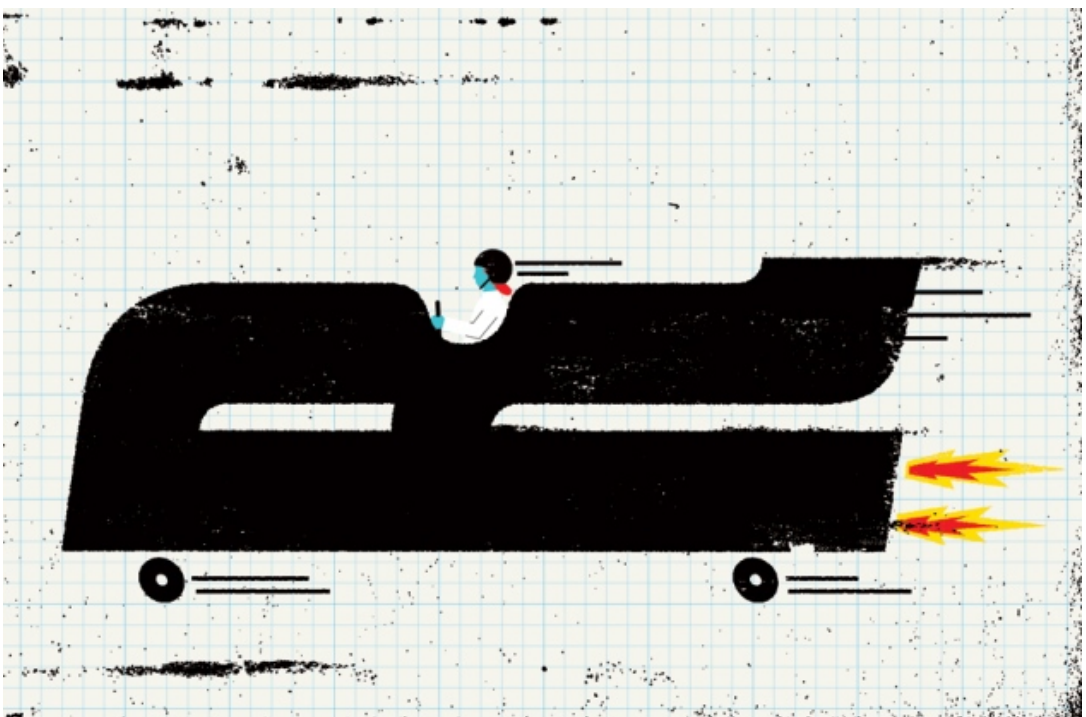
\includegraphics[scale=0.71]{introR.png}
\end{center}
}
\end{frame}


\setbeamercolor{normal text}{fg=black,bg=background}
\begin{frame}[plain]
\hspace*{-1.0cm}\parbox[t]{\textwidth}{
\begin{block}{After this workshop you should be able to:}
\begin{itemize}
\item Understand, create and modify the 4 main objects in R (\code{vector, data.frame, matrix, list}) 
\item Use basic functions
\item Import a dataset from an external file
\item Create a plot
\end{itemize}
\end{block}
}
\end{frame}


\section{1. Background on the R language}

\setbeamercolor{normal text}{fg=gray,bg=black}
\begin{frame}[plain]
\hspace*{-1.0cm}\parbox[t]{\textwidth}{
 \begin{center}
  \Huge{\textcolor{white}{1. Background on the R language}}
 \end{center}
 }
\end{frame}


\setbeamercolor{normal text}{fg=black,bg=background}
\begin{frame}[plain]
\hspace*{-1.0cm}\parbox[t]{\textwidth}{
\begin{block}{Objectives of this section}
\begin{enumerate}
\item Understand the advantages of R
\item Know it's characteristics
\item Start an R session and execute some basic commands
\item Create, modify and save an R script
\end{enumerate}
\end{block}
}
\end{frame}



\setbeamercolor{normal text}{fg=gray,bg=white}
\subsection{The popularity of R}

\begin{frame}
 \begin{center}
  \Huge{\textcolor{red}{The popularity of R}}
 \end{center}
\end{frame}


\begin{frame}{The rise of popularity}

\vspace{0.1in}

\begin{center}
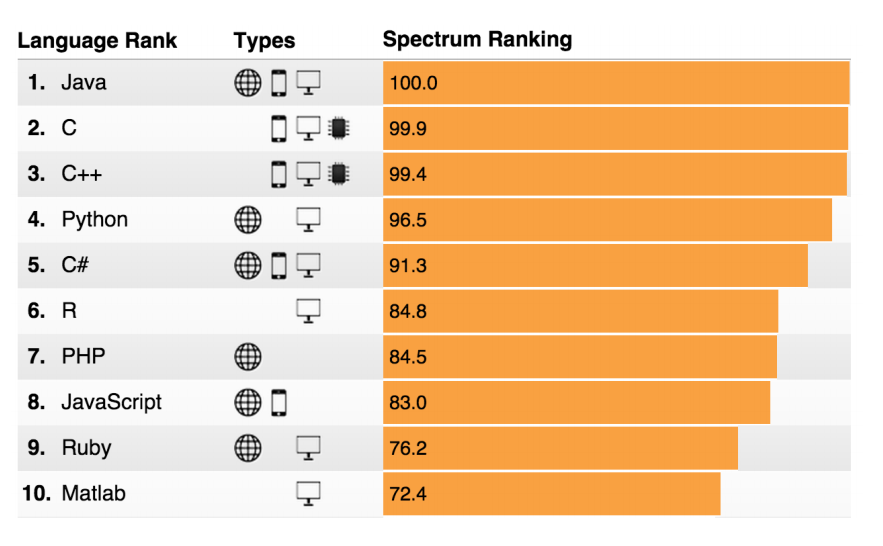
\includegraphics[scale=0.79]{rankings.png}
\end{center}

\vspace{0.2in}

The best programming languages in 2015 according to \href{http://spectrum.ieee.org/computing/software/the-2015-top-ten-programming-languages}{\mbox{IEEE Spectrum}} \\
\end{frame}


\begin{frame}{Number of Jobs}

\begin{center}
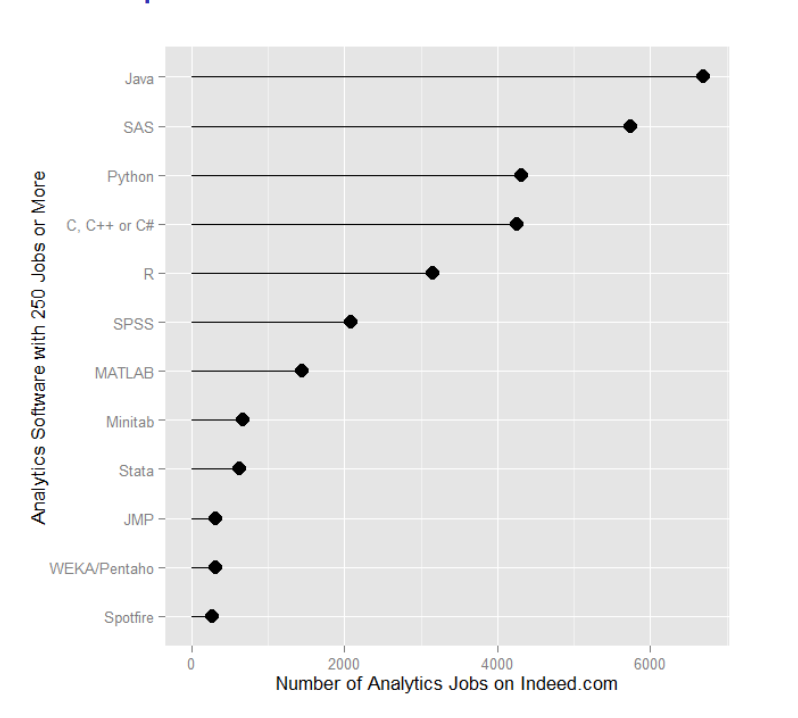
\includegraphics[scale=0.7]{jobs.png}
\end{center}

\vspace{0.05in}

reference: \href{http://r4stats.com/articles/popularity/}{http://r4stats.com/articles/popularity/}\\

\end{frame}



\begin{frame}{Used in many domains}

\begin{center}
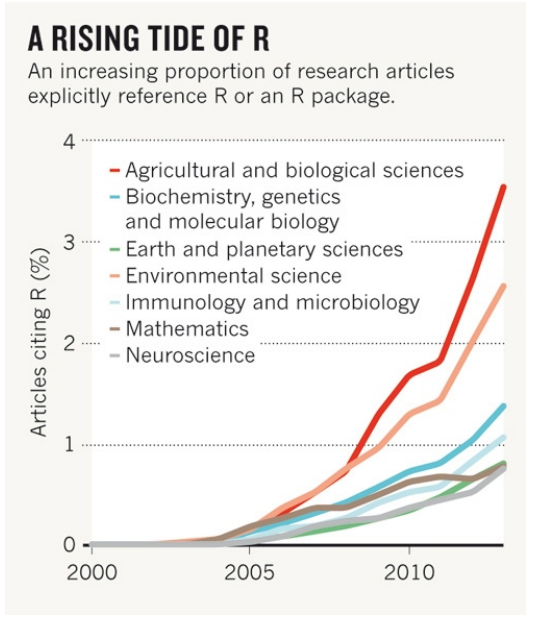
\includegraphics[scale=0.7]{citeR.png}
\end{center}

\vspace{0.05in}

Published in \href{http://www.nature.com/news/programming-tools-adventures-with-r-1.16609}{\textit{Nature}}
\end{frame}


\begin{frame}{Powerful tool to analyze data}
\begin{itemize}
  \setlength\itemsep{2em}
\item Several resources for state-of-the-art statistical computing
\item Powerful graphing system
\item Integrate your R code into web applications
\item Ensure the reproducibility of your analyses
\end{itemize}
\end{frame}



\subsection{A Brief History}

\begin{frame}
 \begin{center}
  \Huge{\textcolor{red}{A Brief History}}
 \end{center}
\end{frame}


\begin{frame}{Before R there was S by John M. Chambers}
\begin{center}
\begin{figure}
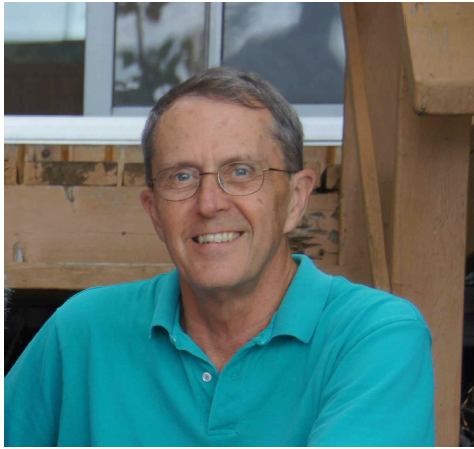
\includegraphics[scale=0.7]{john.png}
\caption{S, is a language developped at Bell Laboratories in the 1970s by a group of researchers led by John M. Chambers}
\end{figure}
\end{center}
\end{frame}


\begin{frame}{Creators of R}
\begin{center}
\begin{figure}
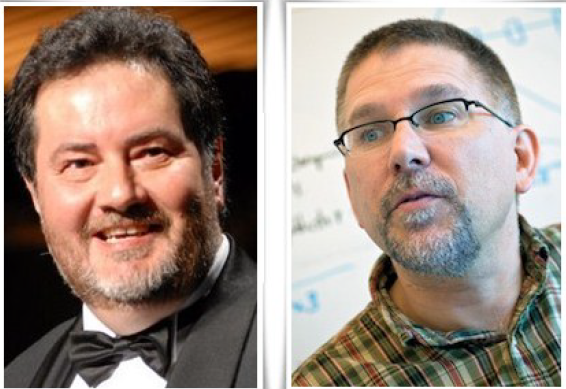
\includegraphics[scale=0.790]{rr.png}
\caption{Inspired by S, Ross Ihaka (left) and Robert Gentleman (right) from the  University of Auckland in New Zeland launched the first version of R in 1996}
\end{figure}
\end{center}
\end{frame}


\begin{comment}
\begin{frame}{Open Source Software}
\begin{itemize}
  \setlength\itemsep{1em}
\item 1990-2010: le S a principalement \'{e}t\'{e} popularis\'{e} par une mise en oeuvre commerciale nomm\'{e}e S-PLUS
\pause \item Fin des ann\'{e}es 2000: L'utilisation de S-PLUS diminue en faveur du R, surtout dans les milieux acad\'{e}miques
\pause \item 2 raisons qui ont fortement contribu\'{e} \`{a} la perte d'influence de S-PLUS
\begin{enumerate}
\item \normalsize Disponible gratuitement
\pause \item Ouvert aux contributions de tous
\end{enumerate}
\end{itemize}
\end{frame}
\end{comment}



\subsection{Characteristics of R}

\begin{frame}
 \begin{center}
  \Huge{\textcolor{red}{Characteristics of R}}
 \end{center}
\end{frame}



\begin{frame}{Object oriented programming language}
\begin{itemize}
  \setlength\itemsep{2em}
\item This makes it easy to find and reuse the results of your analyses
\pause \item A function can complete several tasks
\end{itemize}
\end{frame}


\begin{frame}{An interpreted language}
\begin{itemize}
  \setlength\itemsep{1.2em}
\item An interpreted language: does not require compiling a program into machine-language instructions 
\item A compiled language: \code{C}, \code{C++}, \code{JAVA}
\item More accessible than a compiled language $\rightarrow$ which allows economists, ecologists, biologists, engineers, statisticians, epidemiologists, etc. to use R
\pause \item The program we run to use R is the interpreter
\pause \item This interpreter takes commands in R and it will immediately run
\pause \item Another example: \ code {Python}
\end{itemize}
\end{frame}


\begin{frame}{Open Source Software}

\begin{itemize}
  \setlength\itemsep{1.5em}
\item Active development for the creation of new tools in several fields  
\begin{itemize}
\item \href{https://cran.r-project.org/web/views/}{https://cran.r-project.org/web/views/}
\end{itemize} 
\item Easily see other people's code with GitHub 
\begin{itemize}
\item \href{http://www.r-pkg.org/}{http://www.r-pkg.org/}
\end{itemize}
\item Well-documented with a lot of free resources available on the internet
\begin{itemize}
\item \href{http://stackoverflow.com/questions/tagged/r}{stackoverflow}
\item \href{http://www.rdocumentation.org/}{http://www.rdocumentation.org/} \item \href{http://www.r-bloggers.com/}{http://www.r-bloggers.com/} 
\item \href{https://twitter.com/search?q=\%23rstats}{twitter} 
\item \href{http://blog.revolutionanalytics.com/local-r-groups.html}{R user groups}
\item \href{https://www.google.ca/}{Google}
\end{itemize}
\end{itemize}

%\begin{center}
%\begin{figure}
%\includegraphics[scale=0.35]{meta.png}
%\caption{\href{http://www.r-pkg.org/}{http://www.r-pkg.org/}}
%\end{figure}
%\end{center}

\end{frame}



\begin{frame}[fragile]{Statistical tool that optimizes the matrix approach}

\begin{itemize}
  \setlength\itemsep{2em}
\item The R language is based on the notion of vector, which simplifies mathematical calculations (not only computation but also writing)
\pause \item Reduces the use of iterative structures (loops \code{for, while}, etc.)
\end{itemize}
\pause 
\begin{knitrout}
\definecolor{shadecolor}{rgb}{1, 1, 1}\color{fgcolor}\begin{kframe}
\begin{rcode}\label{unnamed-chunk-1}\begin{alltt}
\hlkwd{c}\hlstd{(}\hlnum{1}\hlstd{,}\hlnum{2}\hlstd{,}\hlnum{3}\hlstd{)} \hlopt{+} \hlkwd{c}\hlstd{(}\hlnum{4}\hlstd{,}\hlnum{5}\hlstd{,}\hlnum{6}\hlstd{)}
\end{alltt}
\begin{verbatim}
## [1] 5 7 9
\end{verbatim}
\end{rcode}\end{kframe}
\end{knitrout}

%\begin{center}
%\begin{figure}
%\includegraphics[scale=0.35]{meta.png}
%\caption{\href{http://www.r-pkg.org/}{http://www.r-pkg.org/}}
%\end{figure}
%\end{center}

\end{frame}





\begin{frame}[fragile]{How to find help for a function}
\begin{itemize}
  \setlength\itemsep{2em}
%\item Pour l'aide g\'{e}n\'{e}ral: \texttt{help.start()} 
%\item Lorsque l'on conna\^{i}t le nom de la commande R: 
%\item \mbox{\texttt{help(nom de la fonction)}} 
\item \mbox{\texttt{?name\_of\_the\_function}}
%\item \`{A} partir des mot-cl\'{e}s: \texttt{??mot cl\'{e}}
%\begin{itemize}
%\item exemple: \code{??regression}
%\end{itemize}
%\item Toutes les commandes fournies par un package: \code{help(package=nom du package)}
%\begin{itemize}
%\item exemple: \code{help(package = datasets)}
%\end{itemize}
%\item F1 sur votre clavier 
\end{itemize}

\pause 
\begin{knitrout}
\definecolor{shadecolor}{rgb}{1, 1, 1}\color{fgcolor}\begin{kframe}
\begin{rcode}\label{unnamed-chunk-2}\begin{alltt}
\hlcom{# find help for linear regression function 'lm'}
\hlopt{?}\hlstd{lm}
\end{alltt}
\end{rcode}\end{kframe}
\end{knitrout}
\end{frame}


\begin{frame}{The help page - 2 main sections}
\begin{itemize}
  \setlength\itemsep{2em}
\item \textbf{Usage:} the name of the function, and all of its arguments and default values
\pause \item \textbf{Value:} the type of object returned and its contents
\end{itemize}
\end{frame}


%\begin{frame}{Clavier Mac}
%\vspace{0.1in}
%\begin{center}
%\includegraphics[scale=0.40]{mackey.jpg}
%\end{center}
%\end{frame}

%\begin{frame}{Clavier PC}
%\vspace{0.1in}
%\begin{center}
%\includegraphics[scale=0.40]{pckey.jpg}
%\end{center}
%\end{frame}



%\subsection{Bref Historique et description}





\subsection{Let's start a session}

\begin{frame}
 \begin{center}
  \Huge{\textcolor{red}{Starting a session}}
 \end{center}
\end{frame}


\begingroup
\makeatletter
\setlength{\hoffset}{-.5\beamer@sidebarwidth}
\makeatother
\begin{frame}[fragile, plain]
\begin{knitrout}
\definecolor{shadecolor}{rgb}{1, 1, 1}\color{fgcolor}\begin{kframe}
\begin{rcode}\label{label}\begin{alltt}
\hlcom{# Start the interface for documentation}
\hlcom{# and navigate the different resources}
\hlkwd{help.start}\hlstd{()}

\hlcom{# find help for the rnorm function}
\hlopt{?}\hlstd{rnorm}

\hlcom{# Get the working directory}
\hlkwd{getwd}\hlstd{()}
\end{alltt}
\end{rcode}\end{kframe}
\end{knitrout}
\end{frame}

%\begin{frame}[fragile, plain]
%<<rcode=TRUE, eval=FALSE>>=
%@
%\end{frame}




\begin{frame}[fragile, plain]
\begin{knitrout}
\definecolor{shadecolor}{rgb}{1, 1, 1}\color{fgcolor}\begin{kframe}
\begin{rcode}\label{unnamed-chunk-3}\begin{alltt}
\hlcom{# addition}
\hlnum{39} \hlopt{+} \hlnum{3}

\hlcom{# substraction}
\hlnum{58} \hlopt{-} \hlnum{16}

\hlcom{# multiplication}
\hlnum{6} \hlopt{*} \hlnum{7}

\hlcom{# division}
\hlnum{8} \hlopt{/} \hlnum{3}
\end{alltt}
\end{rcode}\end{kframe}
\end{knitrout}
\end{frame}



\begin{frame}[fragile, plain]
\begin{knitrout}
\definecolor{shadecolor}{rgb}{1, 1, 1}\color{fgcolor}\begin{kframe}
\begin{rcode}\label{unnamed-chunk-4}\begin{alltt}
\hlcom{# Generate two random vectors of size 50 }
\hlcom{# from a standard normal distribution}
\hlstd{x} \hlkwb{<-} \hlkwd{rnorm}\hlstd{(}\hlnum{50}\hlstd{)}
\hlstd{y} \hlkwb{<-} \hlkwd{rnorm}\hlstd{(}\hlnum{50}\hlstd{)}

\hlcom{# Plot the points (x, y)}
\hlkwd{plot}\hlstd{(x, y)}

\hlcom{# A histogram of x}
\hlkwd{hist}\hlstd{(x)}
\end{alltt}
\end{rcode}\end{kframe}
\end{knitrout}
\end{frame}


\begin{frame}[fragile, plain]
\begin{knitrout}
\definecolor{shadecolor}{rgb}{1, 1, 1}\color{fgcolor}\begin{kframe}
\begin{rcode}\label{unnamed-chunk-5}\begin{alltt}
\hlcom{# to see the contents of the x vector}
\hlstd{x}

\hlcom{# see the objects in your workspace}
\hlkwd{ls}\hlstd{()}

\hlcom{# delete the two vectors x and y}
\hlkwd{rm}\hlstd{(x,y)}

\hlcom{# see the contents of x}
\hlstd{x}

\hlcom{# see the objects in your workspace}
\hlkwd{ls}\hlstd{()}
\end{alltt}
\end{rcode}\end{kframe}
\end{knitrout}
\end{frame}


\begin{frame}[fragile, plain]
\begin{knitrout}
\definecolor{shadecolor}{rgb}{1, 1, 1}\color{fgcolor}\begin{kframe}
\begin{rcode}\label{unnamed-chunk-6}\begin{alltt}
\hlcom{# generate a sequence 1, 2, ..., 20.}
\hlstd{x} \hlkwb{<-} \hlnum{1}\hlopt{:}\hlnum{20}

\hlcom{# create another vector as a function of x}
\hlstd{y} \hlkwb{<-} \hlnum{2} \hlopt{*} \hlstd{x} \hlopt{+} \hlnum{3}

\hlcom{# create a data.frame and see its contents}
\hlstd{dt} \hlkwb{<-} \hlkwd{data.frame}\hlstd{(x, y)}
\hlstd{dt}

\hlcom{# run a linear regression and see the }
\hlcom{# results}
\hlstd{fit} \hlkwb{<-} \hlkwd{lm}\hlstd{(y} \hlopt{~} \hlstd{x,} \hlkwc{data} \hlstd{= dt)}
\hlkwd{summary}\hlstd{(fit)}
\end{alltt}
\end{rcode}\end{kframe}
\end{knitrout}
\end{frame}

\endgroup


\begin{frame}[fragile, plain]
\begin{knitrout}
\definecolor{shadecolor}{rgb}{1, 1, 1}\color{fgcolor}\begin{kframe}
\begin{rcode}\label{unnamed-chunk-7}\begin{alltt}
\hlcom{# The ’seq’ function will generate more general sequences }
\hlkwd{seq}\hlstd{(}\hlkwc{from} \hlstd{=} \hlopt{-}\hlnum{5}\hlstd{,} \hlkwc{to} \hlstd{=} \hlnum{10}\hlstd{,} \hlkwc{by} \hlstd{=} \hlnum{3}\hlstd{)}
\hlkwd{seq}\hlstd{(}\hlkwc{from} \hlstd{=} \hlopt{-}\hlnum{5}\hlstd{,} \hlkwc{length} \hlstd{=} \hlnum{10}\hlstd{)}

\hlcom{#’rep’ repeats values}
\hlkwd{rep}\hlstd{(}\hlnum{1}\hlstd{,} \hlnum{5}\hlstd{)} \hlcom{# repeat 1, 5 times}
\hlkwd{rep}\hlstd{(}\hlnum{1}\hlopt{:}\hlnum{5}\hlstd{,} \hlnum{5}\hlstd{)} \hlcom{# repeat the vector 1,...,5,  five times}
\hlkwd{rep}\hlstd{(}\hlnum{1}\hlopt{:}\hlnum{5}\hlstd{,} \hlkwc{each} \hlstd{=} \hlnum{5}\hlstd{)} \hlcom{# repeat each element five times}
\end{alltt}
\end{rcode}\end{kframe}
\end{knitrout}
\end{frame}



\begin{frame}[fragile, plain]
\begin{knitrout}
\definecolor{shadecolor}{rgb}{1, 1, 1}\color{fgcolor}\begin{kframe}
\begin{rcode}\label{unnamed-chunk-8}\begin{alltt}
\hlcom{# vector arithmetic}
\hlstd{v} \hlkwb{<-} \hlnum{1}\hlopt{:}\hlnum{12}  \hlcom{# initialize a vector}
\hlstd{v} \hlopt{+} \hlnum{2} \hlcom{# add 2 to each element of the vector}
\hlstd{v} \hlopt{* -}\hlnum{12}\hlopt{:-}\hlnum{1} \hlcom{# element-wise product}
\hlstd{v} \hlopt{+} \hlnum{1}\hlopt{:}\hlnum{3} \hlcom{# the shortest vector is recycled}

\hlcom{# Generate random uniform(1,10) numbers }
\hlstd{v} \hlkwb{<-} \hlkwd{runif}\hlstd{(}\hlnum{12}\hlstd{,} \hlkwc{min} \hlstd{=} \hlnum{1}\hlstd{,} \hlkwc{max} \hlstd{=} \hlnum{10}\hlstd{); v}

\hlcom{# You can place the call in parentheses to see the result}
\hlstd{( v} \hlkwb{<-} \hlkwd{runif}\hlstd{(}\hlnum{12}\hlstd{,} \hlkwc{min} \hlstd{=} \hlnum{1}\hlstd{,} \hlkwc{max} \hlstd{=} \hlnum{10}\hlstd{) )}
\end{alltt}
\end{rcode}\end{kframe}
\end{knitrout}
\end{frame}




\begin{frame}[fragile, plain]
\begin{knitrout}
\definecolor{shadecolor}{rgb}{1, 1, 1}\color{fgcolor}\begin{kframe}
\begin{rcode}\label{unnamed-chunk-9}\begin{alltt}
\hlcom{# trouver le répertoire où se trouve le}
\hlcom{# jeux de données 'morley', qui est inclu avec}
\hlcom{# l'installation de R}
\hlstd{filepath} \hlkwb{<-} \hlkwd{system.file}\hlstd{(}\hlstr{"data"}\hlstd{,} \hlstr{"morley.tab"}\hlstd{,}
            \hlkwc{package}\hlstd{=}\hlstr{"datasets"}\hlstd{)}

\hlcom{# importer les données dans un objet appeller 'mm'}
\hlstd{mm} \hlkwb{<-} \hlkwd{read.table}\hlstd{(filepath)}

\hlcom{# Graphique }
\hlkwd{plot}\hlstd{(mm}\hlopt{$}\hlstd{Expt, mm}\hlopt{$}\hlstd{Speed,}
\hlkwc{main}\hlstd{=}\hlstr{"Speed of Light Data"}\hlstd{,} \hlkwc{xlab}\hlstd{=}\hlstr{"Experiment No."}\hlstd{)}

\hlcom{# Terminer la session}
\hlkwd{q}\hlstd{()}
\end{alltt}
\end{rcode}\end{kframe}
\end{knitrout}
\end{frame}
\end{comment}




\section{2. Basics of R}

\setbeamercolor{normal text}{fg=gray,bg=black}
\begin{frame}[plain]
\hspace*{-1.0cm}\parbox[t]{\textwidth}{
 \begin{center}
  \Huge{\textcolor{white}{2. Basics of R}}
 \end{center}
 }
\end{frame}

\setbeamercolor{normal text}{fg=black,bg=background}
\begin{frame}[plain]
\hspace*{-1.0cm}\parbox[t]{\textwidth}{
\begin{block}{Objectives of this section}
\begin{enumerate}
\item Understand what a function is and how to use it
\item Identify the main objects in R: \code{vector, matrix, data frame} and \code{list} 
\item Create and manipulate these objects
\item Import some external datasets \code{.txt} et \code{.csv}
\item Install a \textit{package}
\end{enumerate}
\end{block}
}
\end{frame}



\setbeamercolor{normal text}{fg=gray,bg=white}


\subsection{Functions}

\begin{frame}
 \begin{center}
  \Huge{\textcolor{red}{Functions}}
 \end{center}
\end{frame}



\begin{frame}{Definition of a Function}
\begin{itemize}
 \setlength\itemsep{2em}
\item Instead of writing many repetitive lines of code, we call \textbf{functions} instead
\pause \item A function is characterised by two components
\pause 
\begin{enumerate}
\normalsize
\item It's \textbf{name}: this name allows the user to call the function
\pause \item a \textbf{list of arguments}: this is the information the function needs to return a proper result
\end{enumerate}
\end{itemize}
\end{frame}





\begin{frame}[fragile]{Function syntax}
\begin{itemize}
 \setlength\itemsep{2em}
\item You have to write the name of the function followed by two parentheses
\pause \item The required arguments between these two parentheses are what the function requires to execute it:
\begin{center}
\code{name\_of\_the\_function(arguments)}
\end{center}
\end{itemize}
\pause 
\begin{knitrout}
\definecolor{shadecolor}{rgb}{1, 1, 1}\color{fgcolor}\begin{kframe}
\begin{rcode}\label{unnamed-chunk-10}\begin{alltt}
\hlcom{# look at the help page for square root function}
\hlopt{?}\hlstd{sqrt}

\hlcom{# we see that the sqrt function takes one argument}
\hlkwd{sqrt}\hlstd{(}\hlnum{49}\hlstd{)}
\end{alltt}
\end{rcode}\end{kframe}
\end{knitrout}

\end{frame}



\begin{frame}[fragile]{Optional arguments}
\begin{itemize}
 \setlength\itemsep{0.5em}
\item Certain functions have optional arguments while others have no arguments at all: \code{getwd()}) 
\pause \item The optional arguments have a default value 
\pause \item If we do not specify the optional argument, then the function will use the default, else it will use the argument value specified
\end{itemize}
\pause 

\begin{knitrout}\footnotesize
\definecolor{shadecolor}{rgb}{1, 1, 1}\color{fgcolor}\begin{kframe}
\begin{rcode}\label{unnamed-chunk-11}\begin{alltt}
\hlcom{# look at the help for the logarithm function}
\hlopt{?}\hlstd{log}

\hlcom{# we don't need to specify a value for the 2nd argument }
\hlkwd{log}\hlstd{(}\hlnum{2}\hlstd{)}

\hlcom{# we can specify the second argument if we want}
\hlkwd{log}\hlstd{(}\hlnum{2}\hlstd{,} \hlkwc{base} \hlstd{=} \hlkwd{exp}\hlstd{(}\hlnum{1}\hlstd{))}
\end{alltt}
\end{rcode}\end{kframe}
\end{knitrout}

\end{frame}




\subsection{R Objects}

\begin{frame}
 \begin{center}
  \Huge{\textcolor{red}{R Objects}}
 \end{center}
\end{frame}


%\begin{frame}[<+->]{Les objets R}
%\begin{itemize}
%  \setlength\itemsep{2em}
%\item Tout dans le langage R est un objet:
%\begin{itemize}
%\item les variables contenant des données
%\item les fonctions, 
%\item les opérateurs, même le symbole représentant le nom d’un
%objet est lui-même un objet.
%\end{itemize}
%\end{itemize}
%\end{frame}




\begin{frame}{R Objects}

%\begin{itemize}
%  \setlength\itemsep{2em}
%\item Les structures de données peuvent être organisées par: 
%\pause
%\begin{enumerate}
%\item leur dimension (1d, 2d, ou nd) 
%\item si elles sont homogène ou hétérogène
%\end{enumerate}
%\pause \item Cela donne lieu à 5 types de données les plus souvent utilisées %dans l'analyse des données:
%\end{itemize}
%\pause 
\ctable[caption={The principal R objects and their name},label=tab:table1,pos=h!,doinside=\small]{ccccc}{\tnote{all the elements have to be of the same type}\tnote[b]{the elements can be of different types}
}{
    																\FL
dimension	&  & same type\tmark	    &	& different type\tmark[b] \ML
1d & & Atomic vector & & List \NN
   & &    \code{c()} & & \code{list()} \ML
2d & & Matrix & & Data frame \NN
   & &  \code{matrix()} & & \code{data.frame()} \LL
}

\end{frame}


\begin{frame}[fragile]{\textit{Atomic vectors}}

\begin{itemize}
  \setlength\itemsep{2em}
\item In R, everything is a vector
\pause \item The function to create a vector is \code{c()} (concatenation)
\end{itemize}
\pause
\begin{knitrout}
\definecolor{shadecolor}{rgb}{1, 1, 1}\color{fgcolor}\begin{kframe}
\begin{rcode}\label{unnamed-chunk-12}\begin{alltt}
\hlkwd{c}\hlstd{(}\hlnum{1}\hlstd{,} \hlnum{2}\hlstd{,} \hlnum{5}\hlstd{)}
\end{alltt}
\begin{verbatim}
## [1] 1 2 5
\end{verbatim}
\end{rcode}\end{kframe}
\end{knitrout}

\end{frame}




\begin{frame}[fragile]{\textit{Atomic vectors}}

\begin{itemize}
  \setlength\itemsep{2em}
\item Frequently used \textit{atomic vectors}: 
\begin{enumerate}
\item \textit{double} (also called \textit{numeric})
\item \textit{integer}
\item \textit{character}
\item \textit{logical}
\end{enumerate}
\end{itemize}
\pause
\begin{knitrout}
\definecolor{shadecolor}{rgb}{1, 1, 1}\color{fgcolor}\begin{kframe}
\begin{rcode}\label{unnamed-chunk-13}\begin{alltt}
\hlkwd{c}\hlstd{(}\hlnum{1}\hlstd{,} \hlnum{2.5}\hlstd{,} \hlnum{4.5}\hlstd{)} \hlcom{# numeric}
\hlkwd{c}\hlstd{(}\hlnum{1L}\hlstd{,} \hlnum{6L}\hlstd{,} \hlnum{10L}\hlstd{)} \hlcom{# integer}
\hlkwd{c}\hlstd{(}\hlstr{"these are"}\hlstd{,} \hlstr{"characters"}\hlstd{)} \hlcom{#character}
\hlkwd{c}\hlstd{(}\hlnum{TRUE}\hlstd{,} \hlnum{FALSE}\hlstd{, T, F)} \hlcom{# logical}
\end{alltt}
\end{rcode}\end{kframe}
\end{knitrout}

\end{frame}






\begin{frame}[fragile]{Test}

\begin{itemize}
  %\setlength\itemsep{1em}
\item \code{typeof()}: to find out the type of vector
\item \code{is.character(), is.double(), is.integer(), is.logical(), is.atomic()}: for case specific types 
\end{itemize}
\pause
\begin{knitrout}\footnotesize
\definecolor{shadecolor}{rgb}{1, 1, 1}\color{fgcolor}\begin{kframe}
\begin{rcode}\label{unnamed-chunk-14}\begin{alltt}
\hlstd{int_var} \hlkwb{<-} \hlkwd{c}\hlstd{(}\hlnum{1L}\hlstd{,} \hlnum{6L}\hlstd{,} \hlnum{10L}\hlstd{)}
\hlkwd{typeof}\hlstd{(int_var)}
\end{alltt}
\begin{verbatim}
## [1] "integer"
\end{verbatim}
\begin{alltt}
\hlkwd{is.integer}\hlstd{(int_var)}
\end{alltt}
\begin{verbatim}
## [1] TRUE
\end{verbatim}
\begin{alltt}
\hlkwd{is.atomic}\hlstd{(int_var)}
\end{alltt}
\begin{verbatim}
## [1] TRUE
\end{verbatim}
\end{rcode}\end{kframe}
\end{knitrout}

\end{frame}



\begin{frame}[fragile]{Test}

\begin{knitrout}
\definecolor{shadecolor}{rgb}{1, 1, 1}\color{fgcolor}\begin{kframe}
\begin{rcode}\label{unnamed-chunk-15}\begin{alltt}
\hlstd{dbl_var} \hlkwb{<-} \hlkwd{c}\hlstd{(}\hlnum{1}\hlstd{,} \hlnum{2.5}\hlstd{,} \hlnum{4.5}\hlstd{)}
\hlkwd{typeof}\hlstd{(dbl_var)}
\end{alltt}
\begin{verbatim}
## [1] "double"
\end{verbatim}
\begin{alltt}
\hlkwd{is.double}\hlstd{(dbl_var)}
\end{alltt}
\begin{verbatim}
## [1] TRUE
\end{verbatim}
\begin{alltt}
\hlkwd{is.atomic}\hlstd{(dbl_var)}
\end{alltt}
\begin{verbatim}
## [1] TRUE
\end{verbatim}
\end{rcode}\end{kframe}
\end{knitrout}

\end{frame}


\begin{frame}[fragile]{\textit{Coercion}}

\begin{itemize}
  \setlength\itemsep{1em}
\item All the elements of an \textit{atomic vector} must be of the same type
\pause \item When you try to combine several types, it will convert everything to the most flexible type
\pause \item From least flexible to most flexible:
\begin{enumerate}
\item \textit{logical} 
\item \textit{integer} 
\item \textit{double} 
\item \textit{character}
\end{enumerate}
\end{itemize}
\begin{knitrout}
\definecolor{shadecolor}{rgb}{1, 1, 1}\color{fgcolor}\begin{kframe}
\begin{rcode}\label{unnamed-chunk-16}\begin{alltt}
\hlcom{# combine a character and an interger will produce what?}
\hlkwd{str}\hlstd{(}\hlkwd{c}\hlstd{(}\hlstr{"a"}\hlstd{,} \hlnum{1}\hlstd{))}
\end{alltt}
\begin{verbatim}
##  chr [1:2] "a" "1"
\end{verbatim}
\end{rcode}\end{kframe}
\end{knitrout}
\end{frame}



\begin{frame}[fragile]{\textit{Coercion}}
\begin{itemize}
\item Most mathematical operations will convert an \textit{atomic vector} into a \textit{double} or \textit{integer}
\end{itemize}
\begin{knitrout}\footnotesize
\definecolor{shadecolor}{rgb}{1, 1, 1}\color{fgcolor}\begin{kframe}
\begin{rcode}\label{unnamed-chunk-17}\begin{alltt}
\hlstd{x} \hlkwb{<-} \hlkwd{c}\hlstd{(}\hlnum{FALSE}\hlstd{,} \hlnum{FALSE}\hlstd{,} \hlnum{TRUE}\hlstd{)}
\hlkwd{as.numeric}\hlstd{(x)}
\end{alltt}
\begin{verbatim}
## [1] 0 0 1
\end{verbatim}
\begin{alltt}
\hlcom{# Number of TRUE}
\hlkwd{sum}\hlstd{(x)}
\end{alltt}
\begin{verbatim}
## [1] 1
\end{verbatim}
\begin{alltt}
\hlcom{# Proportion of TRUE}
\hlkwd{mean}\hlstd{(x)}
\end{alltt}
\begin{verbatim}
## [1] 0.33
\end{verbatim}
\end{rcode}\end{kframe}
\end{knitrout}
\end{frame}


\begin{frame}[fragile]{\textit{List}}

\begin{itemize}
  %\setlength\itemsep{2em}
\item \textit{lists} are different from \textit{atomic vectors} because the elements will be of the same type
\item The function to create a \textit{list} is a \code{list()}
\end{itemize}
\pause
\begin{knitrout}\footnotesize
\definecolor{shadecolor}{rgb}{1, 1, 1}\color{fgcolor}\begin{kframe}
\begin{rcode}\label{unnamed-chunk-18}\begin{alltt}
\hlstd{(x} \hlkwb{<-} \hlkwd{list}\hlstd{(}\hlnum{1}\hlopt{:}\hlnum{3}\hlstd{,} \hlstr{"a"}\hlstd{,} \hlkwd{c}\hlstd{(}\hlnum{TRUE}\hlstd{,} \hlnum{FALSE}\hlstd{,} \hlnum{TRUE}\hlstd{),} \hlkwd{c}\hlstd{(}\hlnum{2.3}\hlstd{,} \hlnum{5.9}\hlstd{)))}
\end{alltt}
\begin{verbatim}
## [[1]]
## [1] 1 2 3
## 
## [[2]]
## [1] "a"
## 
## [[3]]
## [1]  TRUE FALSE  TRUE
## 
## [[4]]
## [1] 2.3 5.9
\end{verbatim}
\end{rcode}\end{kframe}
\end{knitrout}

\end{frame}



\begin{comment}
\begin{frame}[fragile]{Attributs}

\begin{itemize}
  %\setlength\itemsep{2em}
\item Les attributs d'un objet sont des éléments d'information additionnels liés à cet objet
\item Pour chaque attribut, il existe une fonction du même nom servant à extraire l'attribut correspondant d’un objet
\end{itemize}

\ctable[caption={Attributs les plus usuels d'un objet},label=tab:table1,pos=h!,doinside=\small]{ccccc}{
}{
    																\FL
Attribut	&  & Utilisation \ML
class & & affecte le comportement d’un objet \\
dim & & dimensions des matrices et tableaux \\
dimnames & & étiquettes des dimensions des matrices et tableaux \\
names & & étiquettes des éléments d’un objet\LL
}
\end{frame}
\end{comment}





\begin{frame}[fragile]{\textit{Matrix}}

\begin{itemize}
  \setlength\itemsep{1em}
\item Matrices are nothing but vectors in 2 dimensions
\pause \item Used for mathematical computations (think of linear algebra courses)
\pause \item The function to create a \textit{matrix} is \code{matrix()}
\end{itemize}
\pause
\begin{knitrout}
\definecolor{shadecolor}{rgb}{1, 1, 1}\color{fgcolor}\begin{kframe}
\begin{rcode}\label{unnamed-chunk-19}\begin{alltt}
\hlcom{# filled by column by defaults}
\hlkwd{matrix}\hlstd{(}\hlkwd{c}\hlstd{(}\hlnum{1}\hlstd{,}\hlnum{2}\hlstd{,}\hlnum{3}\hlstd{,}\hlnum{4}\hlstd{,}\hlnum{5}\hlstd{,}\hlnum{6}\hlstd{),} \hlkwc{nrow} \hlstd{=} \hlnum{2}\hlstd{,} \hlkwc{ncol} \hlstd{=} \hlnum{3}\hlstd{)}
\end{alltt}
\begin{verbatim}
##      [,1] [,2] [,3]
## [1,]    1    3    5
## [2,]    2    4    6
\end{verbatim}
\end{rcode}\end{kframe}
\end{knitrout}

\end{frame}


\begin{frame}[fragile]{\textit{Matrix}}

\begin{knitrout}
\definecolor{shadecolor}{rgb}{1, 1, 1}\color{fgcolor}\begin{kframe}
\begin{rcode}\label{unnamed-chunk-20}\begin{alltt}
\hlcom{# automatically converted to same data type}
\hlkwd{matrix}\hlstd{(}\hlkwd{c}\hlstd{(}\hlnum{1}\hlstd{,}\hlnum{2}\hlstd{,}\hlnum{3}\hlstd{,}\hlstr{"a"}\hlstd{,}\hlstr{"b"}\hlstd{,}\hlstr{"c"}\hlstd{),} \hlkwc{nrow} \hlstd{=} \hlnum{2}\hlstd{,} \hlkwc{ncol} \hlstd{=} \hlnum{3}\hlstd{)}
\end{alltt}
\begin{verbatim}
##      [,1] [,2] [,3]
## [1,] "1"  "3"  "b" 
## [2,] "2"  "a"  "c"
\end{verbatim}
\end{rcode}\end{kframe}
\end{knitrout}

\end{frame}





\begin{frame}[fragile]{\textit{Data frame}}

\begin{itemize}
  \setlength\itemsep{0.5em}
\item The \textit{data frame} is a collection of vectors of different types
%\pause \item Utiliser lorsque différents sortes de données ont étés collecter sur les m\^{e}mes sujets (essaie clinique) 
\pause \item The function to create a \textit{data frame} is \code{data.frame()}
\end{itemize}
\pause
\begin{knitrout}
\definecolor{shadecolor}{rgb}{1, 1, 1}\color{fgcolor}\begin{kframe}
\begin{rcode}\label{unnamed-chunk-21}\begin{alltt}
\hlcom{# an 'id'  column to identify the individuals}
\hlcom{# an 'age' column for their age}
\hlkwd{data.frame}\hlstd{(}\hlkwc{id} \hlstd{=} \hlkwd{c}\hlstd{(}\hlstr{"yi"}\hlstd{,}\hlstr{"yang"}\hlstd{,}\hlstr{"zhengzin"}\hlstd{),}
           \hlkwc{age} \hlstd{=} \hlkwd{c}\hlstd{(}\hlnum{37}\hlstd{,}\hlnum{34}\hlstd{,}\hlnum{32}\hlstd{))}
\end{alltt}
\begin{verbatim}
##         id age
## 1       yi  37
## 2     yang  34
## 3 zhengzin  32
\end{verbatim}
\end{rcode}\end{kframe}
\end{knitrout}

\end{frame}




\begin{frame}[fragile]{The difference between a \textit{data frame} and a \textit{matrix}?}

\begin{itemize}
  \setlength\itemsep{2em}
  \normalsize
\item \code{matrix}: matrix calculations
%\pause \item Utiliser lorsque différents sortes de données ont étés collecter sur les m\^{e}mes sujets (essaie clinique) 
\item \code{data.frame}: all other analyses of different data types
\end{itemize}

\end{frame}




\subsection{R Commands}

\begin{frame}
 \begin{center}
  \Huge{\textcolor{red}{R Commands}}
 \end{center}
\end{frame}


\begin{frame}[fragile]{Expression and Assignment} 
\begin{enumerate}
\item An \textbf{expression} is immediately evaluated and the result is posted in the R console:
\pause
\begin{knitrout}
\definecolor{shadecolor}{rgb}{1, 1, 1}\color{fgcolor}\begin{kframe}
\begin{rcode}\label{unnamed-chunk-22}\begin{alltt}
\hlnum{2} \hlopt{+} \hlnum{3}
\end{alltt}
\begin{verbatim}
## [1] 5
\end{verbatim}
\begin{alltt}
\hlstd{pi}
\end{alltt}
\begin{verbatim}
## [1] 3.1
\end{verbatim}
\begin{alltt}
\hlkwd{cos}\hlstd{(pi}\hlopt{/}\hlnum{4}\hlstd{)}
\end{alltt}
\begin{verbatim}
## [1] 0.71
\end{verbatim}
\end{rcode}\end{kframe}
\end{knitrout}
\seti
\end{enumerate}

\end{frame}


\begin{frame}[fragile]{Expression and Assignment} 
\begin{enumerate}
\conti
\item When performing an \textbf{assignment}, an expression is evaluated, but the result is stored in an object and nothing is printed to the console
\begin{itemize}
\item The assignment operator is <-  
\item the two characters < and - must be placed one after another (no spaces):
\end{itemize}
\pause
\begin{knitrout}
\definecolor{shadecolor}{rgb}{1, 1, 1}\color{fgcolor}\begin{kframe}
\begin{rcode}\label{unnamed-chunk-23}\begin{alltt}
\hlstd{a} \hlkwb{<-} \hlnum{5}
\hlstd{a}
\end{alltt}
\begin{verbatim}
## [1] 5
\end{verbatim}
\begin{alltt}
\hlstd{b} \hlkwb{<-} \hlstd{a} \hlopt{-} \hlnum{2}
\hlstd{b}
\end{alltt}
\begin{verbatim}
## [1] 3
\end{verbatim}
\end{rcode}\end{kframe}
\end{knitrout}
\seti
\end{enumerate}

\end{frame}

\begin{frame}[fragile]{Expression and Assignment} 
\begin{enumerate}
\conti
\item To create an assignment and simultaneously print its result, you can place the expression in parentheses:
\pause
\begin{knitrout}
\definecolor{shadecolor}{rgb}{1, 1, 1}\color{fgcolor}\begin{kframe}
\begin{rcode}\label{unnamed-chunk-24}\begin{alltt}
\hlstd{(a} \hlkwb{<-} \hlnum{2} \hlopt{+} \hlnum{3}\hlstd{)}
\end{alltt}
\begin{verbatim}
## [1] 5
\end{verbatim}
\end{rcode}\end{kframe}
\end{knitrout}
\pause \item The = is valid, but is not recommended
\begin{itemize}
\item it can cause confusion between the \code{name = value} in function calls
\end{itemize}

\end{enumerate}
\end{frame}


\begin{frame}[fragile]{Naming conventions for objects}
\begin{itemize}
  \setlength\itemsep{2em}
\item Characters are allowed for naming objects: 
\begin{enumerate}
\item lower case letters a–z 
\item upper case letters A–Z
\item numbers 0–9, 
\item the period .
\item underscore \_
\end{enumerate}
\end{itemize}

\end{frame}


\begin{frame}[fragile]{Naming conventions}
\begin{itemize}
  \setlength\itemsep{2em}
\item R is case-sensitive, which means \code{foo, Foo} and \code{FOO} are three distinct objects
\pause \item Certain names are reserved for R functions, so its best to avoid them
\begin{center}
\code{c, q, t, C, D, I, diff, length, mean, pi, range, var, sd}\\
\code{break, else, for, function, if, in, next, repeat, return, while}\\
\code{TRUE, FALSE, T, F}\\
\code{Inf, NA, NaN, NULL}
\end{center}
\end{itemize}

\end{frame}



\begin{frame}[fragile]{Indexing a \textit{vector}}
\begin{itemize}
  \setlength\itemsep{2em}
\item Indexing has two purposes
\pause \begin{enumerate}
\normalsize
\item extract elements 
\item replace elements
\end{enumerate}
\end{itemize}
\pause 
\begin{knitrout}
\definecolor{shadecolor}{rgb}{1, 1, 1}\color{fgcolor}\begin{kframe}
\begin{rcode}\label{unnamed-chunk-25}\begin{alltt}
\hlcom{# create a vectir}
\hlstd{x} \hlkwb{<-} \hlkwd{c}\hlstd{(}\hlkwc{a} \hlstd{=} \hlopt{-}\hlnum{1}\hlstd{,} \hlkwc{b} \hlstd{=} \hlnum{2}\hlstd{,} \hlkwc{c} \hlstd{=} \hlnum{8}\hlstd{,} \hlkwc{d} \hlstd{=} \hlnum{10}\hlstd{)}

\hlcom{# extract by position}
\hlstd{x[}\hlnum{1}\hlstd{]}

\hlcom{# extract by name}
\hlstd{x[}\hlstr{"c"}\hlstd{]}

\hlcom{# remplace the second element by 5}
\hlstd{x[}\hlnum{2}\hlstd{]} \hlkwb{<-} \hlnum{5}
\end{alltt}
\end{rcode}\end{kframe}
\end{knitrout}
\end{frame}



\begin{frame}[fragile]{Indexing a \textit{data frame} and a \textit{matrix}}

\begin{itemize}
  \setlength\itemsep{2em}
\item Indexing observations by rows and columns for the \textit{data.frame} and \textit{matrix}:
\begin{center}
\code{df[row, column]}
\end{center}

\end{itemize}
\pause 
\begin{knitrout}\small
\definecolor{shadecolor}{rgb}{1, 1, 1}\color{fgcolor}\begin{kframe}
\begin{rcode}\label{unnamed-chunk-26}\begin{alltt}
\hlcom{# create a data frame}
\hlstd{d} \hlkwb{<-} \hlkwd{data.frame}\hlstd{(}\hlkwc{Noms} \hlstd{=} \hlkwd{c}\hlstd{(}\hlstr{"Pierre"}\hlstd{,} \hlstr{"Jean"}\hlstd{,} \hlstr{"Jacques"}\hlstd{),}
\hlkwc{Age} \hlstd{=} \hlkwd{c}\hlstd{(}\hlnum{42}\hlstd{,} \hlnum{34}\hlstd{,} \hlnum{19}\hlstd{),}
\hlkwc{Fumeur} \hlstd{=} \hlkwd{c}\hlstd{(}\hlnum{TRUE}\hlstd{,} \hlnum{TRUE}\hlstd{,} \hlnum{FALSE}\hlstd{))}

\hlstd{d[}\hlnum{1}\hlstd{, ]} \hlcom{# first row}

\hlstd{d[ ,}\hlnum{1}\hlstd{]} \hlcom{# first column}

\hlstd{d[}\hlnum{3}\hlstd{,}\hlnum{2}\hlstd{]} \hlcom{# third row, second column}
\end{alltt}
\end{rcode}\end{kframe}
\end{knitrout}
\end{frame}




\begin{frame}[fragile]{Indexing a \textit{list}}

\begin{knitrout}
\definecolor{shadecolor}{rgb}{1, 1, 1}\color{fgcolor}\begin{kframe}
\begin{rcode}\label{unnamed-chunk-27}\begin{alltt}
\hlcom{# create a list}
\hlstd{x} \hlkwb{<-} \hlkwd{list}\hlstd{(}\hlkwc{player} \hlstd{=} \hlkwd{c}\hlstd{(}\hlstr{"V"}\hlstd{,} \hlstr{"C"}\hlstd{),}
                  \hlkwc{score} \hlstd{=} \hlkwd{c}\hlstd{(}\hlnum{10}\hlstd{,} \hlnum{12}\hlstd{))}

\hlcom{# first element of the list}
\hlstd{x[[}\hlnum{1}\hlstd{]]}

\hlcom{# 1st element of the 2nd element of the list}
\hlstd{x[[}\hlnum{2}\hlstd{]][}\hlnum{1}\hlstd{]}
\end{alltt}
\end{rcode}\end{kframe}
\end{knitrout}
\end{frame}


\begin{frame}[fragile]{Import data and code}



\ctable[caption={Functions for importing data and code},label=tab:table1,pos=h!,doinside=\small]{lccc}{\tnote{value is separated by a space}\tnote[b]{each value is separated by a comma}\tnote[c]{objects in your working environment}
}{
    																\FL
        	  & files	           &	 objects\tmark[c]  &    R script\ML
import  & \code{read.table()\tmark} &       \code{load()} &   \code{source()}    \NN
          &  \code{read.csv()\tmark[b]}  &                 &                 \ML
save  & \code{write.table()} &  \code{save()} &   File -> Save As..         \NN
             & \code{write.csv()}   &    \LL
} 


\end{frame}


\begin{frame}[fragile]{Import data}
\begin{itemize}
  \setlength\itemsep{2em}
\item You must specify where the data is located on your hard drive
\begin{itemize}
\normalsize
\pause \item \code{getwd()}: to know the working directory
\pause \item \code{setwd()}: to modify the working directory
\end{itemize}
\end{itemize}
\pause 
\begin{knitrout}
\definecolor{shadecolor}{rgb}{1, 1, 1}\color{fgcolor}\begin{kframe}
\begin{rcode}\label{unnamed-chunk-28}\begin{alltt}
\hlcom{# modify working directory}
\hlkwd{setwd}\hlstd{(}\hlstr{"~/git_repositories/npu/data"}\hlstd{)}

\hlcom{# import the files}
\hlcom{# assign it to the 'lung' and 'admit' objects}
\hlstd{lung} \hlkwb{<-} \hlkwd{read.csv}\hlstd{(}\hlstr{"lung.csv"}\hlstd{)}

\hlstd{admit} \hlkwb{<-} \hlkwd{read.table}\hlstd{(}\hlstr{"admit.txt"}\hlstd{)}
\end{alltt}
\end{rcode}\end{kframe}
\end{knitrout}
\end{frame}




\begin{frame}[fragile]{Import code from an R Script}

\begin{knitrout}\small
\definecolor{shadecolor}{rgb}{1, 1, 1}\color{fgcolor}\begin{kframe}
\begin{rcode}\label{unnamed-chunk-29}\begin{alltt}
\hlcom{# modify the working directory}
\hlkwd{setwd}\hlstd{(}\hlstr{"~/git_repositories/npu/script"}\hlstd{)}

\hlcom{# execute the commands of the RScript 'mtcars.R'}
\hlcom{# and show the output}
\hlkwd{source}\hlstd{(}\hlstr{"mtcars.R"}\hlstd{,} \hlkwc{echo} \hlstd{=} \hlnum{TRUE}\hlstd{)}

\hlcom{# save the results in an RData object}
\hlkwd{save}\hlstd{(df, fit,} \hlkwc{file} \hlstd{=} \hlstr{"mtcars.RData"}\hlstd{)}

\hlcom{# delete the R objects}
\hlkwd{rm}\hlstd{(df, fit)}

\hlcom{# import the R objects saved in 'mtcars.RData'}
\hlkwd{load}\hlstd{(}\hlstr{"mtcars.RData"}\hlstd{)}
\end{alltt}
\end{rcode}\end{kframe}
\end{knitrout}
\end{frame}




\begin{frame}[fragile]{Instal \textit{packages} in R}

\begin{itemize}
  \setlength\itemsep{1em}
\item A R \textit{\textbf{package}} is a collection of functions, data and documentation that allows a user to perform other tasks.
\item A list of these packages is available at \url{http://www.r-pkg.org/}
\end{itemize}
\pause
\begin{knitrout}
\definecolor{shadecolor}{rgb}{1, 1, 1}\color{fgcolor}\begin{kframe}
\begin{rcode}\label{unnamed-chunk-30}\begin{alltt}
\hlcom{# install packages for reproducible code}
\hlkwd{install.packages}\hlstd{(}\hlkwd{c}\hlstd{(}\hlstr{"knitr"}\hlstd{,}\hlstr{"rmarkdown"}\hlstd{))}

\hlcom{# to get access to those functions}
\hlkwd{library}\hlstd{(knitr)}
\hlkwd{library}\hlstd{(rmarkdown)}
\end{alltt}
\end{rcode}\end{kframe}
\end{knitrout}
\end{frame}


\subsection{Summary}

\begin{frame}
 \begin{center}
  \Huge{\textcolor{red}{Summary}}
 \end{center}
\end{frame}




\begin{frame}{Summary of basic R commands}
 %\hspace*{-1.9cm}\parbox[t]{\textwidth}{
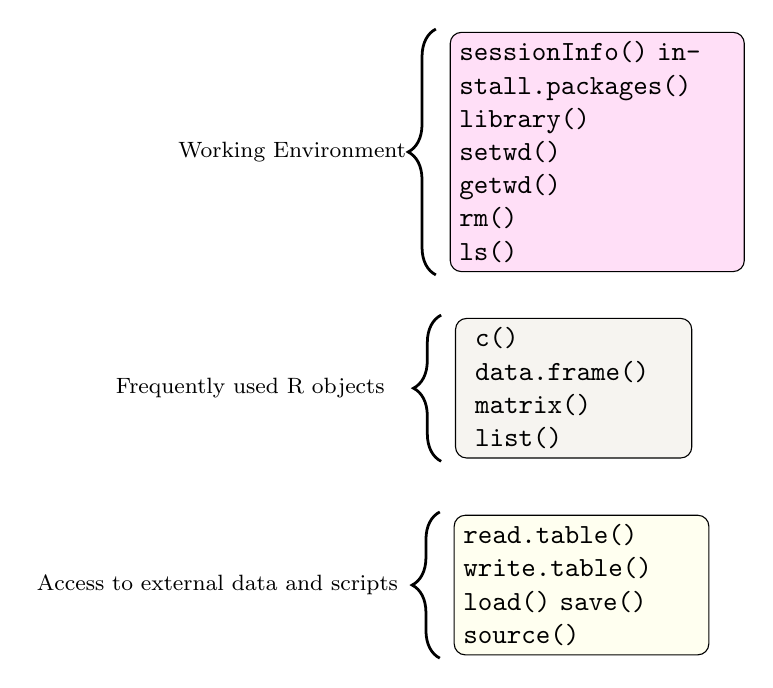
\begin{tikzpicture}
\node (expr) [startstop] {\code{sessionInfo()}
\code{install.packages()}
\code{library()}\textcolor{pinkish}{texxxx}
\code{setwd()}\textcolor{pinkish}{teccc}
\code{getwd()}\textcolor{pinkish}{teccc}
\code{rm()}\textcolor{pinkish}{tevvvvvvv}
\mbox{\code{ls()}\textcolor{pinkish}{tevvvvvvv}}  };
\node (fat) [startstop2, below of=expr, xshift=-.3cm, yshift=-2.0cm] {\code{c()}
\code{data.frame()}
\code{matrix()}
\code{list()}};
\node (script) [startstop3, below of=fat, xshift=.1cm, yshift=-1.5cm] {
\code{read.table()}
\code{write.table()}
\code{load()}
\code{save()}\textcolor{beige}{text}
\code{source()}};
\draw[decoration={brace,raise=5pt, amplitude=10pt},decorate,line width=1pt] 
  ([yshift=-1pt]expr.south west) -- ([yshift=1pt]expr.north west) node [black,midway,xshift=-2cm] 
{\footnotesize Working Environment};
\draw[decoration={brace,raise=5pt,amplitude=10pt},decorate,line width=1pt] 
  ([yshift=-1pt]fat.south west) -- ([yshift=1pt]fat.north west) node [black,midway,xshift=-2.6cm] 
{\footnotesize Frequently used R objects};
\draw[decoration={brace,raise=5pt,amplitude=10pt},decorate,line width=1pt] 
  ([yshift=-1pt]script.south west) -- ([yshift=1pt]script.north west) node [black,midway,xshift=-3cm] 
{\footnotesize Access to external data and scripts};
\end{tikzpicture}
%}
\end{frame}




\section{3. R Graphics}

\setbeamercolor{normal text}{fg=gray,bg=black}
\begin{frame}[plain]
\hspace*{-1.0cm}\parbox[t]{\textwidth}{
 \begin{center}
  \Huge{\textcolor{white}{3. R Graphics}}
 \end{center}
 }
\end{frame}

%\begin{comment}
\setbeamercolor{normal text}{fg=black,bg=background}
\begin{frame}[plain]
\hspace*{-1.0cm}\parbox[t]{\textwidth}{
\begin{block}{Objectives of this section}
\begin{enumerate}
\item Understand the syntax of the\code{plot} function
\item Create \code{boxplot, histogram} and \code{density} plot
\item How to save plots
\end{enumerate}
\end{block}
}
\end{frame}



\setbeamercolor{normal text}{fg=gray,bg=white}
\subsection{The plot function}

\begin{frame}
 \begin{center}
  \Huge{\textcolor{red}{The \code{plot} function}}
 \end{center}
\end{frame}



\begin{frame}[fragile]{Introduction to R graphics}
\begin{itemize}
  \setlength\itemsep{2em}
  \item R offers lots of graphical tools 
  \item To get an idea of what is possible, type the command \code{demo(graphics)} 
\end{itemize}
\end{frame}


\begin{frame}[fragile]{The \code{plot} function}

\begin{itemize}
  \setlength\itemsep{2em}
\item The \code{plot} function can take several different inputs
\end{itemize}
\pause 
\begin{knitrout}
\definecolor{shadecolor}{rgb}{1, 1, 1}\color{fgcolor}\begin{kframe}
\begin{rcode}\label{unnamed-chunk-31}\begin{alltt}
\hlcom{# Plot vector values against the index}
\hlcom{# equivalent to plot(mtcars[,"mpg"])}
\hlkwd{plot}\hlstd{(mtcars}\hlopt{$}\hlstd{mpg,} \hlkwc{xlab} \hlstd{=} \hlstr{"Index"}\hlstd{,} \hlkwc{ylab} \hlstd{=} \hlstr{"mpg"}\hlstd{,}
    \hlkwc{main} \hlstd{=} \hlstr{"Title"}\hlstd{)}

\hlcom{# Scatterplot (x, y)}
\hlkwd{plot}\hlstd{(mtcars}\hlopt{$}\hlstd{mpg, mtcars}\hlopt{$}\hlstd{disp,} \hlkwc{xlab} \hlstd{=} \hlstr{"mpg"}\hlstd{,}
\hlkwc{ylab} \hlstd{=} \hlstr{"disp"}\hlstd{,} \hlkwc{main} \hlstd{=} \hlstr{"mpg vs. disp"}\hlstd{)}
\end{alltt}
\end{rcode}\end{kframe}
\end{knitrout}

\end{frame}


\begin{frame}[fragile]{The \code{plot} function}

\begin{itemize}
  \setlength\itemsep{1.5em}
\item The \code{plot} function can also take a linear model object as input
\pause \item This is an example of how R is an object oriented language
\end{itemize}
\pause 
\begin{knitrout}
\definecolor{shadecolor}{rgb}{1, 1, 1}\color{fgcolor}\begin{kframe}
\begin{rcode}\label{unnamed-chunk-32}\begin{alltt}
\hlcom{# import 'mtcars.RData'}
\hlkwd{load}\hlstd{(}\hlstr{"~/git_repositories/npu/script/mtcars.RData"}\hlstd{)}

\hlcom{# Diagnostic plots for linear model}
\hlcom{# place in 2 rows and 2 columns}
\hlkwd{par}\hlstd{(}\hlkwc{mfrow}\hlstd{=}\hlkwd{c}\hlstd{(}\hlnum{2}\hlstd{,}\hlnum{2}\hlstd{))}
\hlkwd{plot}\hlstd{(fit)}
\end{alltt}
\end{rcode}\end{kframe}
\end{knitrout}

\end{frame}


\subsection{\code{histogram} and \code{boxplot}}

\begin{frame}
 \begin{center}
  \Huge{\textcolor{red}{\code{histogram} and \code{boxplot}}}
 \end{center}
\end{frame}



\begin{frame}[fragile]{The \code{histogram} function}

\begin{itemize}
  \setlength\itemsep{1.5em}
  \item Useful for seeing the data distribution
\item For continuous univariate variables
\end{itemize}
\pause 
\begin{knitrout}
\definecolor{shadecolor}{rgb}{1, 1, 1}\color{fgcolor}\begin{kframe}
\begin{rcode}\label{unnamed-chunk-33}\begin{alltt}
\hlcom{# height for 237 students}
\hlcom{# in the 'survey' data of library(MASS)}
\hlkwd{library}\hlstd{(MASS)}

\hlcom{# see the names of the columns}
\hlkwd{names}\hlstd{(survey)}

\hlcom{# plot histogram of height}
\hlkwd{hist}\hlstd{(survey}\hlopt{$}\hlstd{Height,} \hlkwc{labels} \hlstd{=} \hlnum{TRUE}\hlstd{)}
\end{alltt}
\end{rcode}\end{kframe}
\end{knitrout}

\end{frame}





\begin{frame}[fragile]{The \code{boxplot} function}

\begin{itemize}
  \setlength\itemsep{2em}
\item Useful for seeing if there's a difference between two groups
\end{itemize}
\pause 
\begin{knitrout}
\definecolor{shadecolor}{rgb}{1, 1, 1}\color{fgcolor}\begin{kframe}
\begin{rcode}\label{unnamed-chunk-34}\begin{alltt}
\hlcom{# height for 237 students by gender}
\hlcom{# in the 'survey' data of library(MASS)}

\hlkwd{boxplot}\hlstd{(survey}\hlopt{$}\hlstd{Height} \hlopt{~} \hlstd{survey}\hlopt{$}\hlstd{Sex,}
         \hlkwc{ylab} \hlstd{=} \hlstr{"Height (cm)"}\hlstd{,}
         \hlkwc{col} \hlstd{=} \hlkwd{c}\hlstd{(}\hlstr{"lightpink"}\hlstd{,}\hlstr{"lightblue"}\hlstd{))}
\end{alltt}
\end{rcode}\end{kframe}
\end{knitrout}

\end{frame}


\begin{frame}[fragile]{Saving graphics}

\begin{itemize}
  \setlength\itemsep{2em}
\item 2 main functions: \code{pdf()} and \code{png()}
\item the argument of these functions is the name of the file
\end{itemize}
\pause 
\begin{knitrout}
\definecolor{shadecolor}{rgb}{1, 1, 1}\color{fgcolor}\begin{kframe}
\begin{rcode}\label{unnamed-chunk-35}\begin{alltt}
\hlcom{# enregistrer dans le répertoire de travail courant}
\hlkwd{pdf}\hlstd{(}\hlstr{"boxplot_survey.pdf"}\hlstd{)}
\hlkwd{boxplot}\hlstd{(survey}\hlopt{$}\hlstd{Height} \hlopt{~} \hlstd{survey}\hlopt{$}\hlstd{Sex,}
         \hlkwc{ylab} \hlstd{=} \hlstr{"Height (cm)"}\hlstd{)}
\hlkwd{dev.off}\hlstd{()}
\end{alltt}
\end{rcode}\end{kframe}
\end{knitrout}

\end{frame}



\subsection{Summary}

\begin{frame}
 \begin{center}
  \Huge{\textcolor{red}{Summary}}
 \end{center}
\end{frame}




\begin{frame}{Summary of graphics commands}
 %\hspace*{-1.9cm}\parbox[t]{\textwidth}{
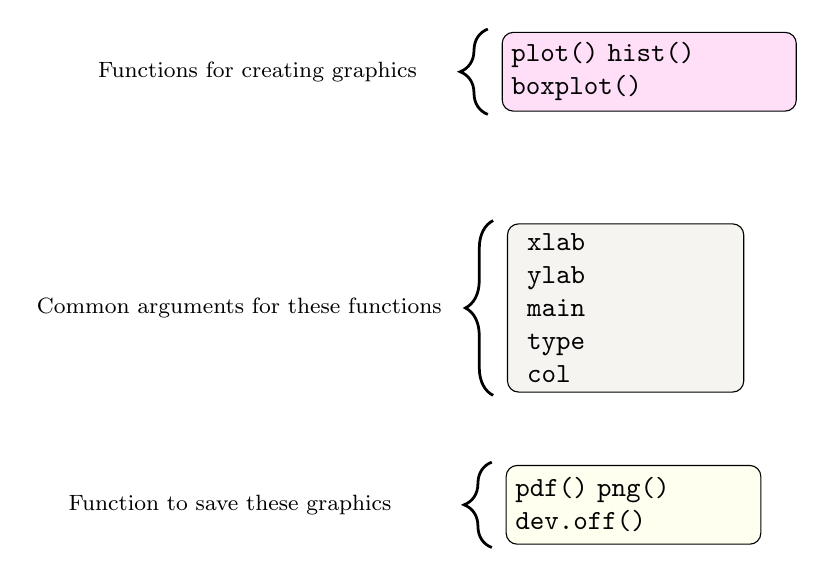
\begin{tikzpicture}
\node (expr) [startstop] {\code{plot()}
\code{hist()}\textcolor{pinkish}{texxxx}
\code{boxplot()}\textcolor{pinkish}{texxxx} };
\node (fat) [startstop2, below of=expr, xshift=-.3cm, yshift=-2.0cm] {\code{xlab}
\code{ylab}\textcolor{background}{textttt}
\code{main}\textcolor{background}{textttt}
\code{type}\textcolor{background}{textttt}
\code{col}\textcolor{background}{textttt}};
\node (script) [startstop3, below of=fat, xshift=.1cm, yshift=-1.5cm] {\code{pdf()}
\code{png()}\textcolor{beige}{textttt}
\code{dev.off()}\textcolor{beige}{textttt}}; 
\draw[decoration={brace,raise=5pt, amplitude=10pt},decorate,line width=1pt] 
  ([yshift=-1pt]expr.south west) -- ([yshift=1pt]expr.north west) node [black,midway,xshift=-3.1cm] 
{\footnotesize Functions for creating graphics};
\draw[decoration={brace,raise=5pt,amplitude=10pt},decorate,line width=1pt] 
  ([yshift=-1pt]fat.south west) -- ([yshift=1pt]fat.north west) node [black,midway,xshift=-3.4cm] 
{\footnotesize Common arguments for these functions};
\draw[decoration={brace,raise=5pt,amplitude=10pt},decorate,line width=1pt] 
  ([yshift=-1pt]script.south west) -- ([yshift=1pt]script.north west) node [black,midway,xshift=-3.5cm] 
{\footnotesize Function to save these graphics};
\end{tikzpicture}
%}
\end{frame}





\section{4. Statistics}

\setbeamercolor{normal text}{fg=gray,bg=black}
\begin{frame}[plain]
\hspace*{-1.0cm}\parbox[t]{\textwidth}{
 \begin{center}
  \Huge{\textcolor{white}{4. Statistiques}}
 \end{center}
 }
\end{frame}

\setbeamercolor{normal text}{fg=gray,bg=white}

\subsection{Mean, Standard Deviation}

\begin{frame}
 \begin{center}
  \Huge{\textcolor{red}{Mean, Standard Deviation}}
 \end{center}
\end{frame}



\begin{frame}[fragile]{Mean, Standard Deviation, Minimum, Maximum}

\begin{itemize}
  \setlength\itemsep{2em}
\item main functions: \code{mean(), var(), sd(), min(), max()}
\pause \item the \code{summary()} function is useful for calculating statistics for a \code{data.frame}
\end{itemize}
\pause 
\begin{knitrout}
\definecolor{shadecolor}{rgb}{1, 1, 1}\color{fgcolor}\begin{kframe}
\begin{rcode}\label{unnamed-chunk-36}\begin{alltt}
\hlkwd{summary}\hlstd{(mtcars)}
\end{alltt}
\end{rcode}\end{kframe}
\end{knitrout}
\end{frame}




\begin{frame}[fragile]{The \code{apply} function}
\begin{itemize}
  \setlength\itemsep{1em}
\item To calculate more complicated summaries of a \textit{data frame} (or \textit{matrix}), we can use the \code{apply} function
\end{itemize}


\end{frame}



\begin{frame}[fragile]{The \code{apply} function}
\begin{itemize}
  \setlength\itemsep{1em}
\item The function syntax is as follows:
\begin{center}
\code{apply(X, MARGIN, FUN)}
\end{center}
\item \code{X}: a matrix or data frame
\item \code{MARGIN}: 1 for rowwise summary, 2 for column wise summary
\item \code{FUN}: is the function to apply
\end{itemize}
\pause 
\begin{knitrout}
\definecolor{shadecolor}{rgb}{1, 1, 1}\color{fgcolor}\begin{kframe}
\begin{rcode}\label{unnamed-chunk-37}\begin{alltt}
\hlcom{# variance by row}
\hlkwd{apply}\hlstd{(mtcars,} \hlnum{1}\hlstd{, var)}
\end{alltt}
\end{rcode}\end{kframe}
\end{knitrout}


\end{frame}









\begin{frame}[fragile]{The \code{apply} function}
\begin{knitrout}
\definecolor{shadecolor}{rgb}{1, 1, 1}\color{fgcolor}\begin{kframe}
\begin{rcode}\label{unnamed-chunk-38}\begin{alltt}
\hlcom{# variance by column}
\hlkwd{apply}\hlstd{(mtcars,} \hlnum{2}\hlstd{, var)}

\hlcom{# sd by column}
\hlkwd{apply}\hlstd{(mtcars,} \hlnum{2}\hlstd{, sd)}

\hlcom{# minimum for each row}
\hlkwd{apply}\hlstd{(mtcars,} \hlnum{1}\hlstd{, min)}


\hlcom{# maximum for each row}
\hlkwd{apply}\hlstd{(mtcars,} \hlnum{1}\hlstd{, max)}
\end{alltt}
\end{rcode}\end{kframe}
\end{knitrout}


\end{frame}





\subsection{t-test and ANOVA}

\begin{frame}
 \begin{center}
  \Huge{\textcolor{red}{t-test and ANOVA}}
 \end{center}
\end{frame}



\begin{frame}[fragile]{t-test}

\begin{itemize}
  \setlength\itemsep{1.5em}
  \item the function for doing a t-test is \code{t.test()}
\end{itemize}
\pause 
\begin{knitrout}
\definecolor{shadecolor}{rgb}{1, 1, 1}\color{fgcolor}\begin{kframe}
\begin{rcode}\label{unnamed-chunk-39}\begin{alltt}
\hlcom{# is there a difference in height between}
\hlcom{# males and females}
\hlkwd{t.test}\hlstd{(Height} \hlopt{~} \hlstd{Sex,} \hlkwc{data} \hlstd{= survey)}
\end{alltt}
\end{rcode}\end{kframe}
\end{knitrout}

\end{frame}







\begin{frame}[fragile]{Analysis of Variance (ANOVA)}

\begin{itemize}
  \setlength\itemsep{2em}
\item The function for ANOVA is \code{aov}
\pause \item Let's take for example the \code{InsectSprays} data in R
\pause \item 6 insecticides were tested 12 times in culture, the response is the number of insects
\pause \item The goal is to see if there is an important difference between the 6 insecticides with respect to the number of insects
\end{itemize}


\end{frame}


\begin{frame}[fragile]{ANOVA}

\begin{knitrout}
\definecolor{shadecolor}{rgb}{1, 1, 1}\color{fgcolor}\begin{kframe}
\begin{rcode}\label{unnamed-chunk-40}\begin{alltt}
\hlcom{# boxplot to see the group difference}
\hlkwd{boxplot}\hlstd{(InsectSprays}\hlopt{$}\hlstd{count} \hlopt{~} \hlstd{InsectSprays}\hlopt{$}\hlstd{spray)}

\hlcom{# Store it in an object called aov.spray}
\hlstd{aov.spray} \hlkwb{<-} \hlkwd{aov}\hlstd{(count} \hlopt{~} \hlstd{spray,} \hlkwc{data} \hlstd{= InsectSprays)}

\hlcom{# see results}
\hlkwd{summary}\hlstd{(aov.spray)}
\end{alltt}
\end{rcode}\end{kframe}
\end{knitrout}

\end{frame}




\subsection{Linear Regression}

\begin{frame}
 \begin{center}
  \Huge{\textcolor{red}{Linear Regression}}
 \end{center}
\end{frame}


\begin{frame}[fragile]{Formulas}

\begin{itemize}
  \setlength\itemsep{1.5em}
  \item Les formules représentent un élément-clé des analyses statistiques avec R
  \pause \item La notation utilisée est la m\^{e}me pour (presque) toutes les fonctions
  \pause \item Une formule est typiquement de la forme 
  \begin{center}
  \code{y $\sim$ model}
  \end{center} 
  \pause \begin{enumerate}
  \item \code{y}: est la réponse analysée 
  \item \code{model}: est un ensemble de termes pour lesquels les paramètres sont estimés
  \end{enumerate}
  \pause \item Ces termes sont séparés par des symboles arithmétiques mais qui ont ici une signification
  particulière: \code{a+b}, \code{a*b}
 \end{itemize}
\end{frame}




\begin{frame}[fragile]{Linear Model}

\begin{knitrout}
\definecolor{shadecolor}{rgb}{1, 1, 1}\color{fgcolor}\begin{kframe}
\begin{rcode}\label{unnamed-chunk-41}\begin{alltt}
\hlcom{# import 'admit.txt'}
\hlstd{admit} \hlkwb{<-} \hlkwd{read.table}\hlstd{(}\hlstr{"admit.txt"}\hlstd{,} \hlkwc{header} \hlstd{=} \hlnum{TRUE}\hlstd{)}

\hlcom{# are gpa and rank related to gre}
\hlstd{fit} \hlkwb{<-} \hlkwd{lm}\hlstd{(gre} \hlopt{~} \hlstd{gpa}\hlopt{+}\hlstd{rank,} \hlkwc{data} \hlstd{= admit)}

\hlcom{# see the results}
\hlkwd{summary}\hlstd{(fit)}
\end{alltt}
\end{rcode}\end{kframe}
\end{knitrout}

\end{frame}


\begin{frame}[fragile]{GLM}

\begin{knitrout}
\definecolor{shadecolor}{rgb}{1, 1, 1}\color{fgcolor}\begin{kframe}
\begin{rcode}\label{unnamed-chunk-42}\begin{alltt}
\hlcom{# logistic regression}
\hlstd{fit.glm} \hlkwb{<-} \hlkwd{glm}\hlstd{(admit} \hlopt{~} \hlstd{gre}\hlopt{+}\hlstd{gpa}\hlopt{+}\hlstd{rank,} \hlkwc{data} \hlstd{= admit,}
           \hlkwc{family} \hlstd{=} \hlkwd{binomial}\hlstd{(}\hlkwc{link} \hlstd{=} \hlstr{"logit"}\hlstd{))}

\hlcom{# see results}
\hlkwd{summary}\hlstd{(fit.glm)}
\end{alltt}
\end{rcode}\end{kframe}
\end{knitrout}

\end{frame}




\subsection{Summary}

\begin{frame}
 \begin{center}
  \Huge{\textcolor{red}{Summary}}
 \end{center}
\end{frame}




\begin{frame}{Summary of Statistics Commands}
 %\hspace*{-1.9cm}\parbox[t]{\textwidth}{
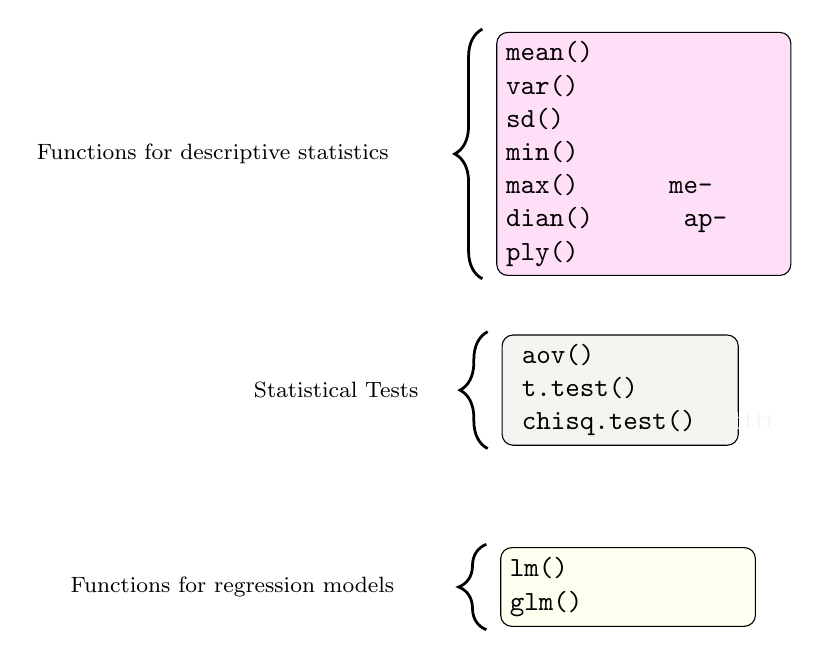
\begin{tikzpicture}
\node (expr) [startstop] {\code{mean()}
\code{var()}\textcolor{pinkish}{texxxxxx}
\code{sd()}\textcolor{pinkish}{texxxx} 
\code{min()}\textcolor{pinkish}{texxxx}
\code{max()}\textcolor{pinkish}{texxxx}
\code{median()}\textcolor{pinkish}{texxxx}
\code{apply()}\textcolor{pinkish}{texxxx}};
\node (fat) [startstop2, below of=expr, xshift=-.3cm, yshift=-2.0cm] {\code{aov()}
\code{t.test()}\textcolor{background}{textttt}
\code{chisq.test()}\textcolor{background}{textttt}};
\node (script) [startstop3, below of=fat, xshift=.1cm, yshift=-1.5cm] {\code{lm()}
\code{glm()}\textcolor{beige}{textdddttt}}; 
\draw[decoration={brace,raise=5pt, amplitude=10pt},decorate,line width=1pt] 
  ([yshift=-1pt]expr.south west) -- ([yshift=1pt]expr.north west) node [black,midway,xshift=-3.6cm] 
{\footnotesize Functions for descriptive statistics};
\draw[decoration={brace,raise=5pt,amplitude=10pt},decorate,line width=1pt] 
  ([yshift=-1pt]fat.south west) -- ([yshift=1pt]fat.north west) node [black,midway,xshift=-2.1cm] 
{\footnotesize Statistical Tests};
\draw[decoration={brace,raise=5pt,amplitude=10pt},decorate,line width=1pt] 
  ([yshift=-1pt]script.south west) -- ([yshift=1pt]script.north west) node [black,midway,xshift=-3.4cm] 
{\footnotesize Functions for regression models};
\end{tikzpicture}
%}
\end{frame}



\section{5. Reproducible Reports}

\setbeamercolor{normal text}{fg=gray,bg=black}
\begin{frame}[plain]
\hspace*{-1.0cm}\parbox[t]{\textwidth}{
 \begin{center}
  \Huge{\textcolor{white}{5. Cr\'{e}er des rapports}}
 \end{center}
 }
\end{frame}

\setbeamercolor{normal text}{fg=gray,bg=white}
\subsection{Introduction}

\begin{frame}
 \begin{center}
  \Huge{\textcolor{red}{Introduction}}
 \end{center}
\end{frame}


\begin{frame}{Introduction}
\begin{itemize}
\item \href{http://rmarkdown.rstudio.com/}{http://rmarkdown.rstudio.com/}
\item \href{http://shiny.rstudio.com/gallery/}{http://shiny.rstudio.com/gallery/}
\end{itemize}
\end{frame}





\begin{frame}[fragile]{Session Information}
\begin{itemize}\raggedright
  \item R version 3.5.0 (2018-04-23), \verb|x86_64-w64-mingw32|
  \item Running under: \verb|Windows 10 x64 (build 17134)|
  \item Matrix products: default
  \item Base packages: base, datasets, graphics, grDevices, methods,
    stats, utils
  \item Other packages: data.table~1.11.0, dplyr~0.7.4,
    ggplot2~2.2.1, knitr~1.20, xtable~1.8-2
  \item Loaded via a namespace (and not attached): assertthat~0.2.0,
    bindr~0.1.1, bindrcpp~0.2.2, colorspace~1.3-2, compiler~3.5.0,
    evaluate~0.10.1, formatR~1.5, glue~1.2.0, grid~3.5.0,
    gtable~0.2.0, highr~0.6, lazyeval~0.2.1, magrittr~1.5,
    munsell~0.4.3, pillar~1.2.2, pkgconfig~2.0.1, plyr~1.8.4,
    R6~2.2.2, Rcpp~0.12.16, rlang~0.2.0, scales~0.5.0, stringi~1.1.7,
    stringr~1.3.0, tibble~1.4.2, tools~3.5.0
\end{itemize}


\end{frame}













\end{document}
